\chapter{Parallel Computing}

The popularity of computational chemistry can be attributed in no small part to the advances and development of highly efficient algorithms in theoretical chemistry. Equally important however is the ever increasing accessibility and performance of computing resources: commercially available work stations can handle chemical systems which could only be modeled on supercomputers a couple decades ago, and firmly cemented the position of computational chemistry as an important "experimental" tool in the toolbox of a chemist. 

As the speed of computers increased over the years, so did the complexity of their components. Nowadays, programmers can choose between several types of architectures, such as shared or distributed memory systems, or accelerators like GPUs. Knowing the strengths and weaknesses of each type is paramount to developing efficient algorithms and tackling larger molecular systems.

This chapter gives an overview on computer architecture, and the different types of parallelism encountered on modern hardware.

\section{Moore's Law}

\emph{Moore's Law} states that the transistor density in integrated chips doubles every 12 to 24 months. First formulated in 1965 by Gordon More, his prediction has held up fairly well over the years. However, the technology enabling this trend has changed over the years.

Figure \ref{fig:MOORE} shows the trends in clock speed, single-thread performance, power consumption and number of logical cores and transistors for microprocessors from 1970 to 2000. Since the early 2000s, clock-speed and single-thread performance have begun to plateau, and have stagnated from 2010 onwards. Increasing the clock speed to values beyond 4 to 5 GHz generates too much stress on the microchip in form of heat, and decreases its performance. This flaw was compensated by using the growing transistor density to instead increase the number of logical cores on a single chip. 

Shifting towards increasing core count however entails that the ideal performance for a CPU can only be achieved though parallel programming. Over the years, the number of different parallel hardware features has drastically increased, and it can be difficult for programmers to fully exploit the available computing resources. Moreover, different programming languages and compiler extensions have emerged as well, with numerous competing standards, especially for GPUs. 

\begin{figure}
\centering
\includegraphics[scale=1.2]{Pics/moore}
\caption[Moore's Law]{Taken from \protect\url{https://github.com/karlrupp/microprocessor-trend-data}}
\label{fig:MOORE}
\end{figure}

\section{Benefits and Limits of Parallel Computing}

While the different available programming models can seem daunting at first, one of the major advantages of parallel computing is improved \emph{scalabilty}. An application that exposes parallelism can be sped up by several orders of magnitude, simply by adding more computing power, with several different architectures to choose from. The limit of what problem sizes can be tackled is mostly dictated by the \emph{amount} of available computing resources and storage, rather than individual processor characteristics.

As important as parallel computing has become in recent years, there is a reason why increasing clock speed was seen as the foremost strategy in keeping Moore's law alive. First, modifying a serial program to exploit parallelism can be a time-consuming endeavor, and second, not all tasks can be effectively parallelized. This means that the potential amount of seed-up is limited by the amount of parallel code. This is known as \emph{Amdahl's law}. The speed-up for a number of cores $N_c$ is given by
\begin{equation}
Speed-Up(N_c) = \frac{1}{S + \frac{P}{N_c}}
\end{equation}
\noindent where $S$ is the fraction of serial code and $P$ is the fraction of parallel code. The speedup for a fixed-size problem as a number of cores is known as \emph{strong scaling}, and the time-to-solution on each individual core \emph{decreases} when more cores are added.

An alternate way to compute potential speed-up is given by Gustafson-Barsis's Law
\begin{equation}
Speed-Up(N_c) = N_c - S(N_c-1)
\end{equation}
\noindent where the problem size also increases proportionally to the number of cores. The scaling for this trend is known as \emph{weak scaling}. In this scenario, the time-to-solution spend on each core remains constant, as the system size and number of cores increases. Even if this type is called "weak", both forms of scaling are equally important, as they address different scenarios. 

\section{Types of Parallelism and Memory Hierarchy}

Nowadays, a programmer has access to four categories of parallelism:
\begin{enumerate}
\item vectorization
\item thread-based parallelism
\item process-based parallelism
\item streaming
\end{enumerate} 
\noindent Leveraging the power of each type requires some understanding of the underlying hardware. 

Figure \ref{clusterArchitecture} shows the major components and memory pathways in a modern computing cluster. A \emph{cluster} is a collection of individual computers that work together and form a single unit. Individual computers are also called \emph{nodes} and occupy a single rack (or "shelf") each in a large server cabinet. The nodes are connected via a low-latency, high through-put network, e.g. Ethernet cables to enable inter-node communication. Each node contains one or more central processing units (CPU) and optionally one or more graphical processing units (GPU). Systems where different types of hardware architecture are mixed are also known as \emph{heterogeneous} systems. The individual components are fixed on a \emph{motherboard}: CPUs are plugged into \emph{sockets} and GPUs into \emph{PCIe slots}. A CPU is composed of one or more cores, where the actual processing of data is carried out. A GPU is also composed of multiple cores, which are grouped into independent \emph{streaming multiprocessors} (SM, NVIDIA), also known as compute units (CU, OpenCL), or subslices (Intel). 

\begin{figure}
\centering
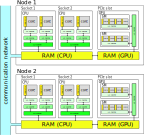
\includegraphics[scale=1.0]{Pics/memory}
\caption{Schematic representation of the architecture of a modern computing cluster which supports heterogeneous computing.}
\label{clusterArchitecture}
\end{figure}

Memory is also a crucial component of computer architecture and is a limited resource. The speed at which data is read from memory can also become a major bottle-neck: No matter how fast a processor is, if the feed rate is too low, it cannot reach its peak performance because it wastes cycles while waiting for data to arrive. To optimize data through-put, the memory model in modern computer architecture requires a complex hierarchy, with different sizes and speeds. Computer memory at the top of the hierarchy has a high response rate, but low complexity. It is also very expensive to produce and therefore much smaller. At the bottom of the hierarchy is memory with large storage space and capable of complex tasks. It is cheap but has low response rate. Over the years, the number of levels in the memory hierarchy has increased. Most modern computers have six levels: CPU registers, L1 cache, L2 cache, L3 cache, DRAM and disk. 

CPU registers sit at the top of the hierarchy and are closest to the cores. It is the region of memory where data is directly manipulated by arithmetic operations and machine code. Its size is typically on the order of several tens to hundreds of bytes. Data is loaded into the registers from \emph{cache}, a region of memory which is further subdivided into different levels named L1, L2 and L3. Each core has its own L1 cache, but might share L2 and L3 cache with other cores. Caches have different sizes and speeds, with L1 being the fastest and smallest at several tens of kB, and L3 being the slowest and largest at several tens to hundreds of kB. Memory is transferred from L3, to L2, to L1 and finally to the CPU registry. The reason why there are multiple levels of cache is to reduce \emph{cache misses}. If data requested by the core is not found in L1, then L2 is searched, then L3. A cache miss is an event where the data is not found anywhere in cache. In that case, a request has to be put out to the dynamical random access memory (DRAM) to retrieve data. Modern techniques such as \emph{cache prefetching} can minimize the amount of cache misses by loading the data into higher cache levels before it is actually needed by the lower levels. 

The speed of DRAM is 10 to 100 time slower than cache, but much larger in size. It is the main memory pool and shared by all cores. CPUs and GPUs have separate DRAM regions which communicate via a PCIe bus. DRAM sizes vary drastically, and are on the order of 10$^0$ to 10$^1$ for GPUs and 10$^0$ to 10$^3$ for CPUs. Data can be transferred from one node to another via CPU DRAM through the communication network, with transfer rates on the order of several GB/s. For programs which are not reading from disk, this is weakest link in the memory hierarchy ???

\section{Vectorization}

Vectorization is the process of operating on multiple variables at the same type. This type of parallelism is encountered at the highest level of the memory hierarchy introduced in the previous section, i.e. CPU registers. Each core has multiple registers, also called \emph{vector registers} with a certain size or \emph{vector length}. Instead of loading each individual element from cache and operating on it, one vector operation on a range of elements can replace multiple single operations. For a 512-bit register, two vectors with 8 floats (32 bit) can be summed within one cycle instead of eight. This type of parallelism is also known as single instruction multiple data (SIMD) in \emph{Flynn's taxonomy}.

The length of vector registers, number of registers as well as the number of supported vector operations have greatly expanded over the years (Table \ref{VECTORHARDWARE}).

\begin{table}
\makegapedcells
\centering
\begin{tabular}{p{0.3\linewidth}cc}
\hline
Release & Vector Length (bit) & No. Registers \\ \hline
SSE (Streaming SIMD Extension) & 128 & 8 \\ 
SSE2/SSE3/SSE4 & 128 & 16  \\
AVX/AVX2 (advanced vector instructions) & 256 & 16 \\
AVX512 & 512 & 32 \\ 
\hline 
\end{tabular}
\caption{Vector lengths and number of registers for commonly encountered vector extensions.}
\label{VECTORHARDWARE}
\end{table}

\subsection{Parallel SAXPY using vectorization}

To show how vectorization can be used in a program, consider the following vector operation:
\begin{equation}
y \leftarrow \alpha x + y
\label{DAXPY}
\end{equation}
\noindent where $y$, $x$ are vectors of equal length, and $\alpha$ is a scaling factor. The vector operation \ref{DAXPY} is also known as "saxpy" for single precision, and "daxpy" for double precision. A naive implementation of the saxpy-kernel is given in Listing \ref{lst:SAXPYNOPARA} for vector size $N$  

\cppcode{Parallelization-unaware implementation of saxpy \label{lst:SAXPYNOPARA}}{listings/saxpy_nopara.c}

\noindent Two arrays are allocated, x and y, and all their entries set to 1 and 2 respectively. Each element is updated individually in the for loop. There are several possibilities to introduce vectorization:
\begin{enumerate}
\item auto-vectorization
\item compiler directives
\item intrinsic functions
\item optimized libraries
\end{enumerate}
\noindent Auto-vectorization is by far the easiest approach: the compiler automatically recognizes that the loop can be vectorized and generates optimized machine code that uses vector instructions. This does not require any input from the user. Compiling the code on a machine with AVX support, using the GNU C compiler, and passing the compiler flags "-O2 -march=native -ftree-vectorize -fopt-info-vec-optimized" generates the following report:
\begin{lstlisting}[backgroundcolor=\color{light-gray},breaklines=true]
saxpy_nopara.c:9:3: optimized: loop vectorized using 32 byte vectors
\end{lstlisting}
\noindent which indicates that the vectors are loaded and operated on in 32 byte chunks, or 8 floats at once. The flag "-ftree-vectorize" (or alternatively "-O3") activates auto-vectorization and "-fopt-info-vec" generates the report. To make sure that the C compiler uses the right vectorization release, the flag "-march=native" is needed, or else the compiler might fall back to SSE. 

In some cases, auto-vectorization cannot take place because the compiler did not recognize that the loop can be vectorized. It can then be beneficial to use \emph{intrinsic functions}. Intrinsic functions are compiler-dependent functions that map to processor operations. When targeting an AVX architecture with 256-bit registers, the saxpy kernel can be rewritten as
\cppcode{SAXPY using intrinsics \label{lst:SAXPYINTRINSICS}}{listings/saxpy_intrinsic.c}
\noindent It is apparent that using intrinsics makes the program much more complex. The arrays cannot be fed directly to the functions, but need to be loaded into vectors of type \texttt{\_\_mm256}, using "set" or "load" functions. Furthermore, the data needs to be aligned correctly using \texttt{\_\_attribute\_\_ ((aligned(...)))}. The arrays are then loaded in chunks into the registers and given to the vector functions for multiplying and adding. 

The major problem with using intrinsic functions, besides increased complexity, is \emph{portability}. The code in \ref{lst:SAXPYINTRINSICS} does not compile on machines that do not support AVX, and is limited to 256-bit registers even on AVX-512 machines. Portable alternatives include using compiler directives or optimized libraries.

Directives (or "pragmas") are hints that can be given to the compiler that suggest that the loop might be vectorizable. By far the most popular set of compiler directives that provide vectorization capabilities is undoubtedly included in the OpenMP application programming interface (API). The OpenMP API is standardized across all compilers, making it highly portable. The OpenMP directives greatly simplify the SAXPY program:
\cppcode{SAXPY using compiler directives \label{lst:SAXPYDIRECTIVES}}{listings/saxpy_simd.c}
\noindent Simply plopping the directive in front of the for loop takes care of generating the appropriate machine code for the targeted architecture. 

The last way to introduce vectorization is via external programs, such as the basic linear algebra subprograms (BLAS) library. It provides a set of specific functions for performing basic vector and matrix operations. Similar to OpenMP, it only provides specifications, and the direct implementation is compiler-dependent. In the BLAS routines, there is a saxpy functions available that can be called directly. It has the advantage of completely removing the loop and clearly states what operation is performed.
\cppcode{SAXPY using BLAS \label{lst:SAXPYBLAS}}{listings/saxpy_blas.c}
\noindent External libraries can however be associated with a steeper learning curve depending on the complexity of function signatures.

\section{Thread-based Parallelism}

Vectorization is limited to single cores only. For multi-core processing, it is important to understand the concept of processes and threads. Processes are executing instances of programs that group related operating system resources together. These resources are exclusive (private) to the process which allocated them, such as system memory, file handles, I/O status information, scheduling information and accounting information. 

A process spawns one or more \emph{threads} (Figure \ref{fig:shared}). A thread is the smallest subset of a process that can be scheduled independently by the OS scheduler. Unlike processes, threads of the same process share resources. They can be seen as "light-weight" processes: start-up of individual threads and communication between threads is much faster. Each core executes only  one thread at a time, but can quickly switch between different threads (or \emph{contexts}). Threads with a higher \emph{priority} are granted more CPU time than threads with lower priority. One a single-core processor, threads are only executed \emph{concurrently}, i.e. they are paused and resumed at regular intervals depending on their priority. On multi-core processors, threads can be executed at the same time (multi-threading), but concurrency is still needed if the number of threads exceeds the number of logical cores.

\begin{figure}[h]
\centering
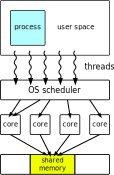
\includegraphics[scale=1.4]{Pics/shared}
\caption{Shared memory parallelism}
\label{fig:shared}
\end{figure}

\subsection{SAXPY using OpenMP}

The most popular standard for thread-based parallelism (or \emph{shared-memory parallelism}) is OpenMP, which was briefly discussed in the previous section. OpenMP was originally introduced to parallelize highly regular loops, but the standard has since then been greatly expanded and includes vectorization directives as well. Using pragmas, multiple threads can be spawned that execute the code within the parallel region. Listing \ref{lst:SAXPYOMP} shows an OpenMP parallel version of SAXPY. Each thread in the parallel region has a unique number associated with it which is used to divide up the arrays. Caution needs to be taken that threads do not operate on the same region at once, as this can lead to undefined behavior ("race conditions").  
\cppcode{SAXPY using OpenMP \label{lst:SAXPYOMP}}{listings/saxpy_omp.c}
\noindent Alternatively, the code may be more easily expressed by using a single compiler directive:
\cppcode{SAXPY using OpenMP \label{lst:SAXPYOMP2}}{listings/saxpy_omp2.c}
\noindent The \texttt{omp parallel for} directive also offers different scheduling tactics which may be difficult to program by hand. Listing \ref{lst:SAXPYOMP} is an example of \emph{static scheduling}, where the work is divided equally among threads \emph{a priori}. However, in the case where each step requires different computational cost, \emph{dynamic scheduling} offers a more balanced approach, although with a somewhat higher prefactor. Threads request tasks, or a chunk of multiple tasks, from the main thread, which distributes work on a first-come first-serve basis. There are many more directives available in the OpenMP standard with a lot of options for fine-tuning. For further details, the reader is referred to the official specifications \cite{OMP2021}.
% (ref) https://www.openmp.org/specifications/

OpenMP is not the only option available for introducing shared-memory parallelism into a program. Alternatives include the \texttt{pthread} (POSIX threads) library for C, the \texttt{std::thread} library, or the Intel TBB (thread building blocks) library for C++. While these libraries can offer a more fine-grained control of threads, the learning curve can be very steep, and parallelizing an application can be very time-consuming. In contrast to OpenMP, they are not based on high-level compiler directives, but rather expose low-level functions and structures that create and control threads. 

Shared-memory parallelism, as the name implies, is limited to cores sharing the same memory space. The primary disadvantage of this model is scalability. It becomes increasingly expensive to produce shared memory systems with more and more cores. Moreover, a larger number of cores implies heavier CPU traffic and time penalties due to \emph{cache coherence}. Cache coherence is the mechanism by which uniformity of data is guaranteed and propagated among processes. There can be multiple copies of the same memory region in cache, which is operated on by different cores. Checking how to combine data from different caches can become costly for a large number of cores.

\section{Process-based Parallelism}

One of the most scalable approaches in parallel computing is process-based parallelism, also known as distributed memory parallelism. Multiple copies of the same program run on separate processes, each with their own local memory and instruction set. In contrast to threads, processes cannot exchange data via shared memory, but need to communicate via a network using \emph{message passing}. The increased cost of communication is often outweighed by the increased potential for scalability. Larger problems can be tackled simply by adding more nodes. 

Pure message-passing assigns or \emph{binds} one rank to a single CPU core. In hybrid parallel approaches, a single process can be bound to a whole node, using shared-memory parallelism for intra-node communication and message passing for inter-node communication. It is also possible to spawn more processes than there are available cores: in that case, the processes are scheduled and executed concurrently similar to threads.

The most popular standard for message passing is the message passing interface (MPI). It defines a set of functions that allow processes to send and receive messages. There are different implementations of MPI, such as the open-source implementations OpenMPI, MPICH, or the vendor implementations Intel MPI or Cray MPI. MPI programs are run using a special start-up command:
\begin{lstlisting}[backgroundcolor=\color{light-gray},breaklines=true]
mpirun -n <nprocs> ./myprogram.exe 
\end{lstlisting}
\noindent The exact command and options depends on the MPI implementation. The start-up program is responsible for duplicating the program on the different processes and establishing the communication network. Most implementations use the flag \texttt{-n} to pass the number of processes to be spawned. 

All processes are characterized by their \emph{rank}, a unique, portable identifier, normally an integer between $[0:nprocs-1]$. Only processes using the same \emph{communicator} can exchange messages. A communicator is a special handle of type \texttt{MPI{\_}Comm} and describes a group of processes. Communicators may also have different \emph{topologies}, such as Cartesian grids, or  graphs, which restrict the flow communication between processes to nearest neighbors. Cartesian grids for example are best suited for matrix operations. By passing topology information to MPI, it can optimize the runtime environment by renumbering tasks such that processes are physically closer to reduce communication overhead. By default, the topology is undefined, and any processor can exchange messages with all other processors.

\subsection{SAXPY using MPI}

Modifying programs to exploit distributed parallelism requires significant effort, with the most crucial point being how data is distributed over the processes. Consider again the SAXPY kernel. There are two memory models: either every process has a copy of the whole array, or the arrays are distributed in chunks over all processes. If data is duplicated on every rank, this can quickly exhaust memory resources for large data sets. On the other hand, if data is distributed in a non-ideal way, commutation may incur major overhead. A programmer has to balance the benefits of data duplication and network communication. 

Listing \ref{lst:SAXPYMPI} shows a distributed memory approach to the SAXPY kernel
\cppcode{SAXPY using MPI \label{lst:SAXPYMPI}}{listings/saxpy_mpi.c}
\noindent The program starts by initializing the executing environment using \texttt{MPI{\_}Init}, and defining the communicator handle. The communicator that groups all processes at start-up is called \texttt{MPI{\_}COMM{\_}WORLD}, and is a macro defined in the header \texttt{<mpi.h>}. If the program is stand-alone, it is safe to use as the primary communicator. When writing a library that is used in combination with other MPI libraries, it is crucial to use a communicator that is passed from the main program. There are two reasons for this: (1) the user may want to use a subcommunicator, rather than the whole process group, and (2) MPI messages have a unique identifier (integer) and if another library uses the same identifier, erroneous communication can take place. In this example, the global communicator is sufficient.

Each process then allocates a local array of size \texttt{num{\_}local} $<$ \texttt{ARRAY{\_}SIZE}. In this example, the main data is initialized on rank 0, which is then split into equal chunks and send to the other processes' local array using \texttt{MPI{\_}Scatter}. Each process then only needs to perform the SAXPY operation on its local chunk. Afterwards, the results are collected on rank 0 using the routine \texttt{MPI{\_}Gather}. Data is then available on rank 0 to be further manipulated, written to console, etc. 

It should be noted that the above program only works for a number of processes that is a divisor of \texttt{ARRAY{\_}SIZE}, because \texttt{MPI{\_}Scatter} and \texttt{MPI{\_}Gather} can only handle chunks that are of equal size on each process. If that is not the case, one can use the more general routines \texttt{MPI{\_}Scatterv} and \texttt{MPI{\_}Gatherv} which also take the different chunk sizes as an input.

Furthermore, the local SAXPY for-loop can be parallelized using the techniques described in the previous sections (vectorization, threads) in case where a process is bound to a whole node and has access to further compute resources.

This program shows only a few of the many functions available for message passing. The MPI standard defines many more functions for sending, receiving, broadcasting, reduction, one-sided communication etc. The official document for the newest MPI standard \cite{MPI2021} is over a thousand pages long, and is updated regularly. Message passing has a very steep learning curve, and can be quite difficult to debug.  

% ref https://www.mpi-forum.org/docs/

\subsection{MPI and Shared Memory}

One may come under the impression that MPI is not efficient on shared-memory systems, as data is exchanged via network-calls. However, MPI is optimized to recognize shared memory and data is then copied within DRAM rather than send through a communication layer, making MPI competitive even on single nodes. Of course, there is still a slight overhead associated with it compared to thread-based parallelism.

MPI standards of version 3.0 and above furthermore introduce functions to allocate shared memory, also known as \emph{windows}, for processes on the same node. Processes can then read/write to the same memory region without using network calls, much in the same manner as OpenMP. This approach can be seen as a MPI+MPI hybrid parallel approach rather than the more frequently used MPI+OpenMP approach. Hybrid parallelism is much more efficient than "MPI-everywhere" approaches due to reduced communication overhead and easier load-balancing. 

MPI+MPI has the advantage of only needing one programming model for both distributed and shared memory access, with relatively easy syntax. However, MPI+MPI is much lesser known, and there are is no automatic support for splitting up loops or atomic loads/stores to shared memory. An external library that offers auxiliary functions for MPI+MPI would be beneficial.

\section{Stream Processing}

The last type of parallelism tackled in this chapter is \emph{stream processing}. A stream is defined as a sequence of data that requires similar (low-level) computation. Streams are processed by \emph{accelerators}, special hardware components with high data throughput, that complement the general purpose CPU by speeding up certain operations. 

\subsection{GPU Architecture}

By far the most popular type of accelerators are graphical processing units (GPUs). As the name implies, GPUs were originally conceived to speed up graphics-related computation, but their use was later extended to include non-graphics workloads as well, in what is known as \emph{general-purpose} graphic processing unit (GPGPU) programming. Nowadays, computing clusters increasingly come with one or more GPGPUs included on each node.

The hardware architecture design of modern GPUs is much more varied than that of CPUs. GPU vendors, like NVIDIA or AMD, have different hardware variations and use different terminology for similar components, and it can be difficult to abstract hardware as some vendor-specific features need to be omitted. Figure \ref{fig:gpu} shows a simplified block diagram of the most common GPU components. A GPU is composed of multiple compute units (CUs), also known as streaming multi-processors (SMs) in NVIDIA GPUs. Work is assigned to different CUs by a workload distributor. Each CU is further subdivided into an array of processing elements (PEs), or CUDA cores as referred to by NVIDIA. A single PE can operate on multiple data elements at once using SIMD or a variation known as single instruction multiple threads (SIMT) used in CUDA cores.

The overall performance of a GPU is given by the number of CUs and PEs, as well as the bandwidth of the PCIe land connecting CPU and GPU. Data transfer between the two devices is often the time-determining step.

\begin{figure}
\centering
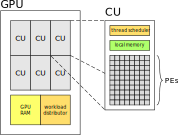
\includegraphics[scale=2.0]{Pics/gpu}
\caption{GPU architecture}
\label{fig:gpu}
\end{figure}

\subsection{GPU Programming Model}

The rise of GPGPU programming has given rise to a plethora of different programming languages and models. Low-level languages like CUDA, OpenCL or HIP directly reflect features of the targeted GPU hardware as part of their syntax, and the user is responsible for managing each aspect of parallelism and data transfer. They require a very thorough understanding of how GPUs operate. Due to the complexity of "native" languages, higher-level languages have gained popularity over the years. Pragma based languages like OpenACC or OpenMP offer a much easier approach to GPU programming that resembles shared memory parallelism on CPUs, and offer a higher degree of portability, at the cost of lower performance ceiling.

Low level languages all operate on a similar programming model which allow the programmer to define special functions called \emph{kernels}, which, when called on a GPU, are executed $N$ times in parallel by $N$ GPU threads. Rather than using for loops, kernels operate on a whole range of data at once, known as a \emph{grid} or NDRange. A grid can be one, two or three-dimensional to allow a more intuitive view of the data at hand. Each grid is subdivided into blocks or work groups which can be executed independently. The maximum size of a block is given by the number of threads in a CU. "Good" values are generally 128, 256 or 512, but the optimal size depends on the hardware and the problem addressed. Threads in a block share memory which is useful in case data from neighboring subblocks is needed. Information on grid and block dimensions are needed by the kernels for distributing work over the GPU.

As an example, consider the SAXPY function using the CUDA programming language:
\cppcode{SAXPY using CUDA \label{lst:SAXPYCUDA}}{listings/saxpy_cuda.cu}
\noindent CPU and GPU do not share memory. The first steps therefore involve allocating memory using \texttt{cudaMalloc} and copying data from CPU ("Host") to GPU ("Device") with the function \texttt{cudaMemcpy}. The arrays can then be passed to the kernel. The kernel function is indicated by the identifier \texttt{\_\_ global\_\_}, and is executed at the same time by all threads in a block. Each thread has a unique block and thread id which indicate its position in the work group. This information is used to make sure that the thread is operating on the correct portion of the array. The GPU threads do not have any information of the loop extent, and it is the user's responsibility to make sure that threads do not write past the allocated memory window by introducing boundary checks (\texttt{if (i < N)}).

In this example for a 1D array, the kernel takes two launch parameters: the number of blocks, and the block size which are put between \texttt{<<< .... >>>} after the function call. Afterwards, the data can be copied back to the CPU for further processing. 

The concept of operating relative to thread coordinates rather than using a for loop with a single index can be quite confusing. Nowadays, there are directive-based compiler extensions, that allow to easily offload work to accelerators, such as OpenMP and OpenACC (Open ACCelerators). Listing \ref{lst:SAXPYACC} shows how a for loop can be easily modified using OpenACC
\cppcode{SAXPY using OpenACC \label{lst:SAXPYACC}}{listings/saxpy_acc.c}
\noindent OpenACC offers several pragmas for allocating and copying arrays to GPUs and back. By only adding two directives, the SAXPY code is easily ported to GPUs. 

\subsection{When to Use GPUs}

Despite the success of GPU computing, GPUs only complement, rather than replace CPUs. GPU cores are very light-weight and have a limited instruction set compared to CPU cores, making them ill-suited for \emph{task-based parallelism}, e.g. running an operating system with many different processes executing in the background. The strength of GPUs rather lies in \emph{data-based parallelism}. Generally, any code that can benefit from vectorization can be sped up using GPUs. 
